% !Mode:: "TeX:UTF-8"
%% 请使用 XeLaTeX 编译本文.
\documentclass{WHUResearch}  % 选项 forprint: 交付打印时, 建议加上此选项, 以消除彩色链接文字, 避免彩色字迹打印偏淡.
                             % 选项 forlib: 提交给图书馆的电子版, 需要加上选项 forlib, 以消除空白页和彩色链接.
                             % 选项 smd: Specialist Master's Degree, 产生专业硕士学位论文封面、页眉.                                                                                                   
%%%=== 参考文献=== %%%
\bibliographystyle{abbrv}    % 参考文献样式,  plain,unsrt,alpha,abbrv 等等
%%%%%%%%%%%%%%%%%%%%%%%%%%%%%%%%%%%%%%%%%%%%%%%%%%%%
\begin{document}
%%%%%%%-------------------------------------------------

\title{Nordic nRF5 开发文档}
\author{钱隆}
\StudentNumber{2019106190015}   % 学号

%-----------------------------------------------------------------------------
\pdfbookmark[0]{封面}{title}         % 封面页加到 pdf 书签
\maketitle
%-----------------------------------------------------------------------------
\pagenumbering{Roman}               % 正文之前的页码用大写罗马字母编号.

\cleardoublepage
\newpage  \pagestyle{fancy} \fancyfancy
%------------------------------------------------------------------------------
%---把目录加入到书签---%%%%%%%%%%%%%%
\pdfbookmark[0]{目录}{toc}%%%%%%%%%%%%

\tableofcontents

%------------------------------------------------------------------------------
\mainmatter %% 以下是正文
\baselineskip=20pt  % 正文行距为 20 磅
\zihao{-4}
%%%%%%%%%%%%%%%%%%%%%%%%%%%%%%%%%%%%
\chapter{Nordic nRF5系列产品开发流程}

These sections will guide you through choosing the right protocols to production programming and testing your product design.

\section{Available protocols}




\chapter{Nordic nRF5系列软件开发环境搭建}

\section{Windows平台基于ARM Keil MDK开发环境搭建}

本节参考\href{https://www.cnblogs.com/iini/p/9043565.html}{iini的博客} \upcite{BKY_iini} 以及 Nordic 的官方入门教程 \href{https://infocenter.nordicsemi.com/index.jsp?topic=\%2Fug_gsg_keil\%2FUG\%2Fgsg\%2Fintro.html&cp=1_1_1}{nRF5 Series: Developing on Windows with ARM Keil MDK},记录在 Windows 平台上基于 ARM Keil MDK 进行 nRF5 系列开发软件环境的准备工作,为今后基于该芯片的开发提供指导。

首先简要介绍一下软件开发环境的依赖项包括:ARM C/C++ 编译器(Compiler),µVision 集成开发环境(Integrated Development Environment)以及 Nordic 官方提供的 nRF5 软件开发工具包(Software Development Kit)。本节所记录的开发环境配置基于 nRF52811 。

\subsection{基础环境配置要求(Minimum Requirements)}

$\bigstar$ 硬件要求

nRF5 系列开发平台(Development Kit, DK)包括一块与之相对应的开发板以及开发板上的芯片。因为Nordic Semiconductor的一些软件开发工具会针对特定的开发板或芯片,所以在进行基于自定义开发板的软件开发之前,需要明确自定义开发板、芯片、SDK等组件的兼容性关系,以确保开发程序正确烧制到自定义开发板上。在相应芯片的说明文档中可以找到对应的兼容矩阵说明。

\href{https://infocenter.nordicsemi.com/index.jsp?topic=\%2Fcomp_matrix_nrf52811\%2FCOMP\%2Fnrf52811\%2Fnrf52811_comp_matrix.html&cp=3_2_2}{nRF52811 平台的兼容性矩阵}(Compatibility Matrix)信息如下:

$\star$ \href{https://infocenter.nordicsemi.com/index.jsp?topic=\%2Fcomp_matrix_nrf52811\%2FCOMP\%2Fnrf52811\%2Fnrf52811_ble_qdid_qual_matrix.html&cp=3_2_2_4}{集成电路修订和变量(IC revisions and variants)}
\begin{table}[htbp]
  \centering
  \caption{nRF52811 IC revisions and variants}
  \begin{threeparttable}
	\begin{tabular}{|c|c|c|c|c|c|}
	\hline
   \textbf{nRF52811 IC revision}  & \textbf{Packet variant}\tnote{1} & \textbf{Build code}\tnote{1} & \textbf{Package} & \textbf{Flash} & \textbf{RAM} \\ \hline
	\multirow{3}{*}{Engineering A} & QFAA 						   & \multirow{3}{*}{AA0} & QFN48 & \multirow{6}{*}{192kB} & \multirow{6}{*}{24kB} \\ \cline{2-2} \cline{4-4}
                  					  & QCAA                     &                   	& QFN32 &                   &                   \\ \cline{2-2} \cline{4-4}
                  					  & CAAA							&                   	& WLCSP &                   &                   \\ \cline{1-4}
	\multirow{3}{*}{\underline{1}} & QFAA							& \multirow{3}{*}{AX0} & QFN48 &                   &                   \\ \cline{2-2} \cline{4-4}
                  					  & \underline{QCAA	}			&                   	& \underline{QFN32} &                   &                   \\ \cline{2-2} \cline{4-4}
                 					  & CAAA							&                   	& WLCSP &                   &                   \\ \hline
	\end{tabular}
	\begin{tablenotes}
	  \footnotesize
        \item[1] Packet variant 和 Build code 可以通过 nRF52 芯片上的印刷标志(N52811 QCAAAA 1836AA)获得。
	\end{tablenotes}
  \end{threeparttable}
\end{table}

$\star$ \href{https://infocenter.nordicsemi.com/index.jsp?topic=\%2Fcomp_matrix_nrf52811\%2FCOMP\%2Fnrf52811\%2Fnrf52811_ble_qdid_qual_matrix.html&cp=3_2_2_4}{软件开发工具包和无线协议栈(SDKs and SoftDevices)}
\begin{table}[htbp]
  \centering
  \caption{nRF52811 IC revisions, nRF5 SDKs, and SoftDevices}
	\begin{tabular}{|c|c|c|c|}
	\hline
 	\multirow{2}{*}{\textbf{nRF52811 IC revision}} & \multirow{2}{*}{\textbf{nRF5 SDK}} &  \multicolumn{2}{c|}{\textbf{BLE}} \\ \cline{3-4}
 															  &  											 & \textbf{S112 SD} & \textbf{S112 SDS} \\ \hline
 	Engineering A; 1 									  & 15.3.0 									 & 6.1.1 				 & 2.2 \\ \hline
	\end{tabular}
\end{table}

$\star$ \href{https://infocenter.nordicsemi.com/index.jsp?topic=\%2Fcomp_matrix_nrf52811\%2FCOMP\%2Fnrf52811\%2Fnrf52811_ble_qdid_qual_matrix.html&cp=3_2_2_4}{硬件开发板(Development HW)}

 nRF52811 开发平台基于 nRF52840 (PCA10056)开发平台。

$\star$ \href{https://infocenter.nordicsemi.com/index.jsp?topic=\%2Fcomp_matrix_nrf52811\%2FCOMP\%2Fnrf52811\%2Fnrf52811_ble_qdid_qual_matrix.html&cp=3_2_2_4}{蓝牙低功耗合格设计标识(Bluetooth Low Energy QDIDs)}
\begin{table}[htbp]
  \centering
  \caption{nRF52811 QDIDs}
	\begin{tabular}{|c|c|}
	\hline
  	\textbf{SoftDevice	} & \textbf{QDID} \\ \hline
  	S112 v6.1.x   	     & TBD \\ \hline
	\end{tabular}
\end{table}

\begin{table}[htbp]
  \centering
  \caption{nRF52840 QDIDs}
	\begin{tabular}{|c|c|c|}
	\hline
	\multicolumn{2}{|c|}{\textbf{SoftDevice}} & \multirow{2}{*}{\textbf{QDID}} \\ \cline{1-2}
  			 \textbf{BLE} & \textbf{ANT \& BLE} &                   \\ \hline
  			 S140 v6.0.0	& \multirow{3}{*}{}  & 108621 \\ \cline{1-1} \cline{3-3} 
  			 S140 v6.1.0	&                    & 115277 \\ \cline{1-1} \cline{3-3} 
  			 S140 v6.1.1	&                    & 124988 \\ \hline
  							& S340 v6.1.1 		  & 124988 \\ \hline
	\end{tabular}
\end{table}

\subsection{开发工具链配置(Setting up your toolchain)}

$\bigstar$ 强制安装项

$\star$ \href{http://www2.keil.com/mdk5/}{Keil MDK-ARM Development Kit}

ARM Keil MDK 包括 ARM C/C++ 编译器以及 µVision IDE。官网上免费下载的 MDK-Lite edition 版本会限制代码大小为 32Kbyte,所以暂时使用破解版µVision V5.23.0.0 IDE,使用 MDK-ARM Professional 许可,安装包包括 IDE 本体和注册机。

\begin{figure}[htbp]
\centering
  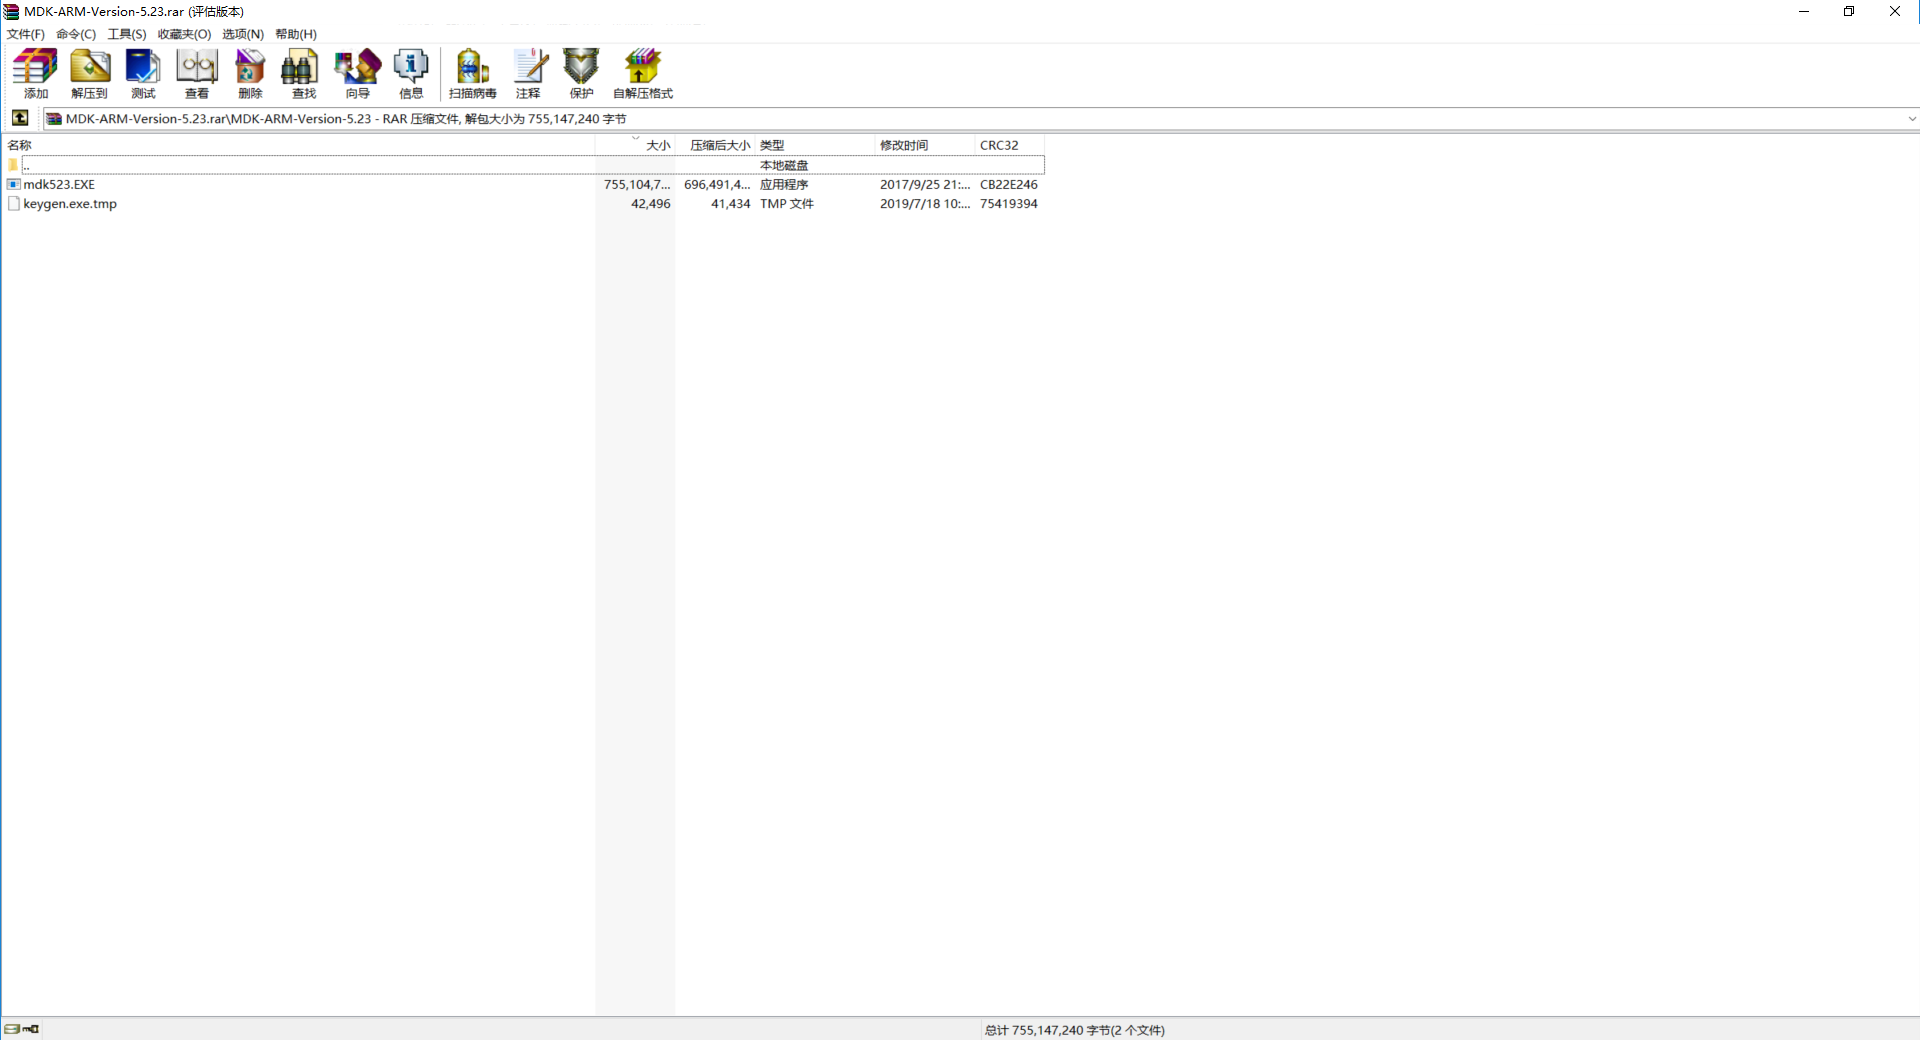
\includegraphics[width=1.0\textwidth]{ARMKeilMDKInstaller.png}
  \caption{ARM Keil MDK 安装包}
  \label{fig:ARMKeilMDKInstaller}
\end{figure}

按照正常流程安装 IDE 本体,安装完本体之后

$\star$ \href{https://developer.nordicsemi.com/}{nRF5 SDK}

$\star$ \href{https://www.nordicsemi.com/Software-and-Tools/Development-Tools/nRF5-Command-Line-Tools/Download#infotabs}{nRF5x Command Line Tools (including nrfjprog)}

$\bigstar$ 可选安装项

\subsection{编写嵌入式程序(Programming an application)}

\subsection{建立开发板通讯(Communicating with the board)}

\subsection{测试嵌入式程序(Testing the application)}

%%%=== 参考文献 ========%%%
\cleardoublepage\phantomsection
\addcontentsline{toc}{chapter}{参考文献}
\begin{thebibliography}{000}\zihao{5}

  \bibitem{BKY_iini} 博客园.Nordic nRF51/nRF52开发环境搭建[Z].iini,2018.  
  
\end{thebibliography}

\cleardoublepage
\end{document}



